% !TEX root = ../thesis-example.tex
%
\chapter{Implementierung}
\label{sec:impl}

Dieses Kapitel behandelt die Implementierung der RapidMiner-Erweiterung \textit{postagger}. Zuerst wird grob auf den technischen Rahmen seitens RapidMiner eingegangen, dann werden im Abschnitt \ref{sec:impl:aims} Ziele der Implementierung angesprochen. \\
Nach einer Übersicht in Abschnitt \ref{sec:impl:structure} über die Komponenten, die Funktionen aus Kap. \ref{sec:concept} implementieren, werden die Komponenten einzeln im Detail vorgestellt.

\section{RapidMiner}
\label{sec:impl:rm}
:TODO(Aufbau auf Text Processing!)
:TODO(Large Lizenz)

Die Datenverarbeitungs-Plattform RapidMiner (kurz \textit{RM}) ist in Java geschrieben, und Erweiterungen dafür ebenfalls. RapidMiners Code ist Open Source und Erweiterungen basierend auf dort definierten Strukturen sind erwünscht. RapidMiners zentrale Funktionalität ist es, verschiedene Funktionen (\textit{Operatoren}) in einem Modell hintereinanderzuschalten und mit ihnen Daten zu extrahieren und mit verschiedensten Mitteln zu transformieren oder zu untersuchen. Ein Beispiel-Prozess von RapidMiner findet sich in Abbildung :TODO(Bild:bsp-Prozess).

\paragraph{Operatoren} 
funktionieren entfernter betrachtet wie Funktionen in herkömmlichem Code: Sie nehmen beliebig viele Eingaben mittels \textit{InputPorts} und \textit{Parametern} entgegen, führen eine Aufgabe aus und haben mindestens eine Ausgabe in Form von \textit{OutputPorts}. Alle Operatoren erben von Superklasse \textit{Operator}. Eine Erweiterung fügt in der Regel solche Operatoren hinzu.
\paragraph{IO-Objekte}
bzw. IOObjects sind die Datenformate im RM-Modell. Sie werden von der Prozesswurzel sowie von Operatoren ausgegeben und können von Operatoren sowie dem Prozess-Ende entgegengenommen werden. Sie erben von der Klasse \textit{IOObject} und können ebenfalls von Erweiterungen hinzugefügt werden. Operatoren können für ihre Inputs definieren, welche Typ von IOObject sie verlangen und das Modell ist nicht lauffähig, wenn diese Spezifikation nicht eingehalten wird.

Für eine ausführliche Dokumentation von RM siehe :NC(Doku), für eine Anleitung zum erstellen von Erweiterungen :NC(your own Extension)


\section{Ziele}
\label{sec:impl:aims}
Diese Erweiterung soll u.A. vom auftraggebenden Lehrstuhl weiterverwendet und -entwickelt werden können. Das heißt, eine gute Dokumentation und Strukturierung der Komponenten steht im Vordergrund. Da die Erweiterung nicht unbedingt von Programmierern benutzt werden soll, muss außerdem auf eine niedrige Fehleranfälligkeit der Implementierung geachtet werden.
\subsection{Erweiterbarkeit}
\subsection{Robustheit}


\section{Übersicht}
\label{sec:impl:structure}

:TODO neues Diagramm! 
\begin{figure}[htb]
	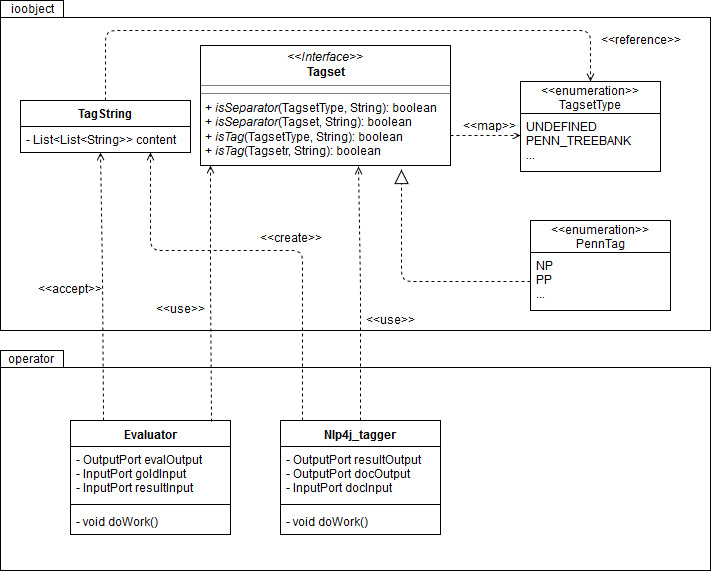
\includegraphics[width=\textwidth]{gfx/UML_Overview_simple.jpg}
	\caption{gekürztes Klassendiagramm}
	\label{fig:impl:structure:overview:uml}
\end{figure}

Abbildung \ref{fig:impl:structure:overview:uml} zeigt einen Überblick über die implementierten Klassen. Um das Diagramm überschaubar zu halten, wurden nur die Klassen eingezeichnet, die zusätzlich zum Erweiterungs-Template von RapidMiner :NC implementiert wurden. Außerdem wurden nur die notwendigen Enumerationen und Klassen für den NLP4J-Tagger aufgenommen, da andere Tagger analog strukturiert sind. Es folgt eine kurze Erklärung der verschiedenen Komponenten:

\paragraph{Operatoren:} \textit{Evaluator} und \textit{Nlp4j\_ tagger} sowie alle anderen Klassen, die von der RapidMiner-Klasse \textit{Operator} erben, sind auch in RapidMiner als Operatoren vertreten. Alle Operatoren außer Evaluator beinhalten einen POS-Tagger und überbrücken sowohl Ein- als auch Ausgangsformate zwischen dem externen RapidMiner-Modell (\textit{Document} oder \textit{TagString} ) und dem Tagging-Algorithmus selbst. Der Evaluator berechnet die Unterschiedlichkeit zwischen zwei Ergebnissen, wobei eines der beiden bestenfalls vollständig korrekt ist. :TODO

\paragraph{Tagsets:} Das Interface Tagset muss von jeder Tag-Enumeration, wie zum Beispiel dem der Penn-Treebank implementiert werden. Zusätzlich bietet es statische Methoden, die die Werte der Enumeration TagsetType auf die korrespondierenden Enumerationen abbilden, sowie Abfragen über deren Werte anbieten (hierzu wird der Typ sowie ein Tag verlangt). Die implementierenden Tagsets führen alle Part-of-Speech-Tags auf und liefern zusätzlich die Information, ob das Tag in der Datenstruktur \textit{TagString} (s.u.) Zeilen abbricht. Auf diese Weise ist es leicht, das Projekt um ein neues Set zu erweitern.

\paragraph{TagString:} Diese Klasse bietet, wie in Abschnitt \ref{sec:impl:plan:thru} angesprochen, ein einheitliches Format für POS-Tags. Sie beschreibt den Tagset-Typen sowie die Zahl an N-Besten Tags pro Token (1 für First-Best) und strukturiert die Tags in Zeilen, die immer dann enden, wenn das letzte Tag ein \textit{Separator} ist. :TODO

\section{Tagsets}

\section{Eingabe und Tokenization}

\section{Ergebnisformat}

\section{Implementierte Tagger}

\section{Evaluations-Operator}
\label{sec:impl:eval}
Um Ergebnisse hinsichtlich ihrer Qualität zu prüfen, muss mit Goldstandards wie z.B. dem WSJ-Corpus :NC verglichen werden. Der Evaluationsoperator muss die Formate dieser Standards annehmen und interpretieren können. Neben dem eigentlichen Evaluieren ist also auch das \textit{Parsen} eingehender Texte eine wichtige Aufgabe des Operators. 

\subsection{Parsing}
\label{sec:impl:eval:parsing}
Verschiedene Formate kodieren POS-Tags unterschiedlich. Eine einfache Notation ist die bereits bekannte Variante, bei der nach jedem Token ein \glqq \textbackslash \grqq{} und dann das Tag folgt. Andere Notationen kodieren zusätzlich Satzstrukturinformationen, sind also mittels Klammern geschachtelt, um z.B. Teilsätze zu markieren. Hier gibt es kein Symbol, das eindeutig ein POS-Tag ankündigt. Um die Parser-Methode des Evaluationsoperators präziser arbeiten können zu lassen, wurde ein Parameter hinzugefügt, in dem man das Format wählen kann. Es wurden zwei Modi für den Parser implementiert:

\paragraph{Backslash-Notation:} In der oben genannten Notation, in der ausschließlich POS via \glqq \textbackslash \grqq{} markiert werden, ist Parsing einheitlich. Der Text wird an jedem Leerzeichen gespalten und jeder entstehende Substring am \glqq \textbackslash \grqq{}. Das POS-Tag findet sich dann im zweiten String, der bei der zweiten Spaltung entsteht.

\paragraph{"None":} Falls die Notation unbekannt ist, versucht der Parser, den Text an allen sinnvollen Symbolen, insbesondere dem Leerzeichen zu Trennen. Alle Substrings werden dann überprüft, ob sie ein POS-Tag sind. 

Zusätzlich kann die Option \textit{\glqq Ignore Brackets \grqq{}} gewählt werden, falls Klammern für die Formatierung des einzulesenden Textes verwendet wurden. diese werden dann ignoriert.
\\
Als Ergebnis gibt der Parser das Format TagString aus, das dann weiter verwendet werden kann. Der Tagset-Typ des TagStrings muss via Parameter angegeben werden.

\section{Conclusion}
\label{sec:system:conclusion}

